\documentclass{beamer}

\usepackage{
    hyperref,
    multicol,
    soul,
    minted,
    xcolor,
    subfig,
    wrapfig,
}
\definecolor{LightGray}{gray}{0.9}
\setbeamercovered{transparent}
\graphicspath{{figures}}

\setlength{\columnsep}{0mm}

\title{A Simple Parcel Theory Model of Downdrafts in Atmospheric Convection}
\author{
    Thomas Schanzer
    \texorpdfstring{\\}{}
    \small \texorpdfstring{
        \url{https://github.com/tschanzer/taste-of-research-21T3}}{
        https://github.com/tschanzer/taste-of-research-21T3
    }
    \texorpdfstring{\\ \vspace{5mm}}{}
    Supervisor: Prof. Steven Sherwood}
\institute{UNSW School of Physics}
\date{Monday 22 November 2021}

\begin{document}

\frame{\titlepage}

\begin{frame}
    \frametitle{Aim and Motivation}
    Downdrafts play an important role in the dynamics of the Earth's
    atmosphere and climate.
    \begin{block}{Question}
        Which processes and conditions initiate, and which
        maintain or inhibit, downdrafts?
    \end{block}
    \begin{block}{Motivation}
        \vspace{-8mm}
        \begin{figure}[ht]
            \centering
            \subfloat[\centering
                Convection parametrisation in global climate models]{
                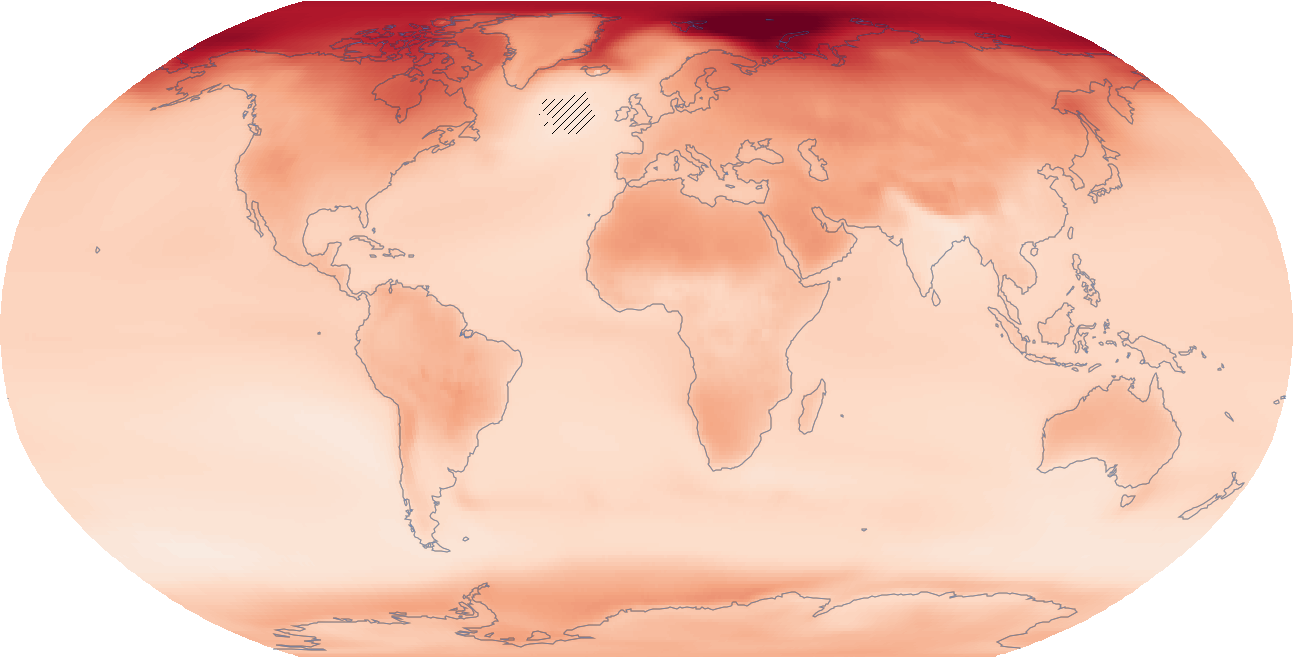
\includegraphics[height=2.5cm]{%
                    figures/ipcc_model_temp_cropped.png}
            }
            \subfloat[\centering
                Forcasting dangerous microbursts]{
                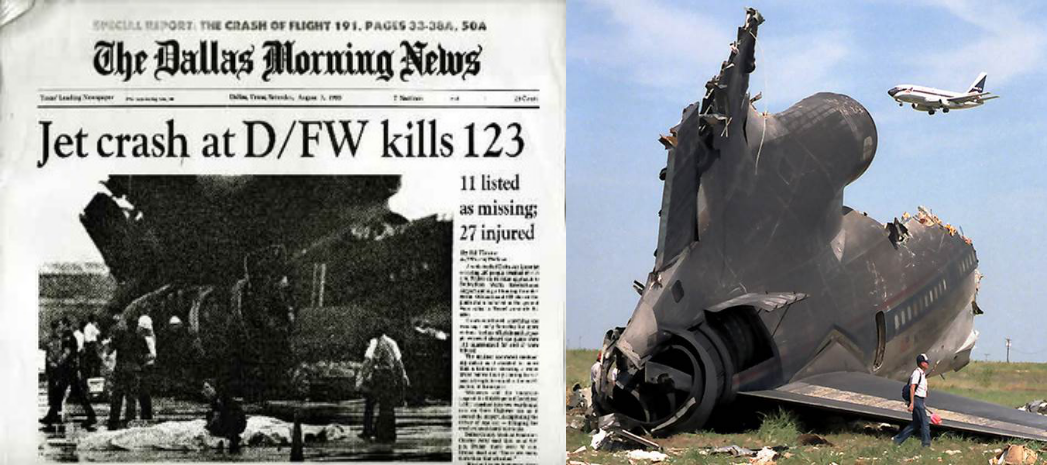
\includegraphics[height=2.5cm]{figures/delta191_side.png}
            }
        \end{figure}
        \tiny \color{gray} (a): IPCC AR6 interactive atlas.
        (b): US National Weather Service.
    \end{block}
\end{frame}

\begin{frame}
    \frametitle{Literature}
    \emph{Knupp and Cotton (1985)}
    \footnote{ \tiny
        Knupp, KR \& Cotton, WR 1985, ‘Convective cloud downdraft
        structure: An interpretive survey’, Reviews of geophysics (1985),
        vol. 23, no. 2, pp. 183–215.}
    identify four downdraft types:
    \vspace{-2mm}
    \begin{multicols}{2}
        \small
        \begin{itemize}
            \item Precipitation-associated (PR)
            \item Penetrative (P)
            \item Cloud-edge (E)
            \item Overshooting (O)
        \end{itemize}
    \end{multicols}
    \vspace{-3mm}
    \begin{figure}[ht]
        \centering
        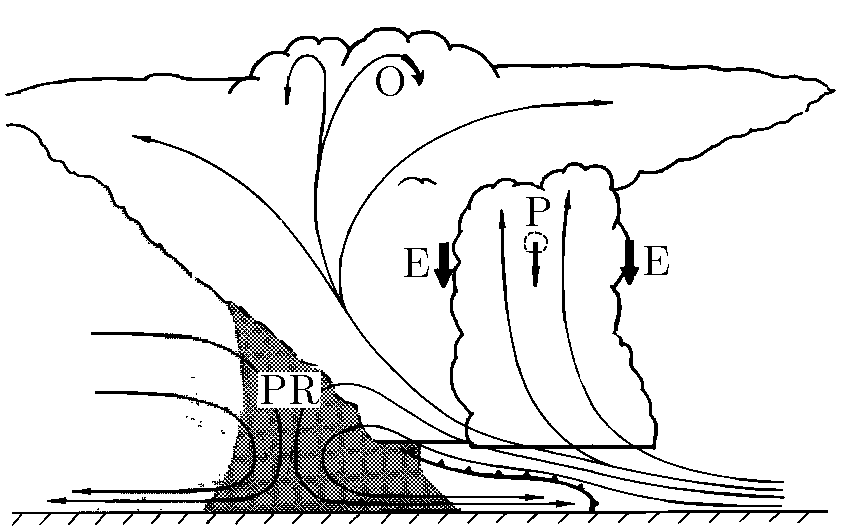
\includegraphics[width=0.6\linewidth]{figures/knupp_cotton_types.pdf}
    \end{figure}
    \vspace{-3mm}
    \centering \tiny Adapted from \emph{Knupp and Cotton (1985)}.
\end{frame}

\begin{frame}
    \frametitle{Background: Parcel Theory}
    \uncover<1>{
    \textbf{Parcel:} small air mass with an imaginary, flexible
    boundary.
    \begin{itemize}
        \item Motion is purely vertical and buoyancy is the only force
            involved:
            \[b = (\text{force/mass})
            = \frac{
                (\text{environment density})
                - (\text{parcel density})
            }{
                (\text{parcel density})
            }g.\]
        \item Raising and lowering the parcel is an adiabatic
            process
    \end{itemize}
    }

    \uncover<2>{
    \textbf{Complication 1:} the atmosphere contains water!
    \begin{itemize}
        \item Descent is either \emph{dry adiabatic} (no phase changes) or
            \emph{moist adiabatic} (with phase changes)
    \end{itemize}
    }
\end{frame}

\begin{frame}[fragile]
    \frametitle{Methods}

    \uncover<1>{
    Original model developed in Python.

    \textbf{Complication 2:} finding the temperature of an
    \emph{entraining} parcel
    \begin{itemize}
        \item Small steps: (non-adiabatic) mixing $\to$
            adiabatic descent $\to$ mixing $\to$ ...
    \end{itemize}
    }

    \uncover<2>{
    End goal: calculate parcel temperature $\to$ density $\to$
    buoyancy as functions of height and numerically solve
    \[\frac{d^2 z}{dt^2} = b(z).\]
    }

    \uncover<3>{
    We can use \emph{any} real or idealised profiles of environmental
    temperature and moisture.
    }
\end{frame}

\begin{frame}
    \frametitle{Results: Precipitation Enhances Downdrafts}
    \begin{figure}[ht]
        \centering
        \includegraphics[width=0.9\linewidth]%
            {figures/motion_vs_initial_conditions_50RH_1perkm.eps}
    \end{figure}
\end{frame}

\begin{frame}
    \frametitle{Results: Entrainment Inhibits Downdrafts}
    \begin{figure}[ht]
        \centering
        \includegraphics[width=0.9\linewidth]%
            {figures/motion_vs_entr_rate_2gram_50RH.eps}
    \end{figure}
\end{frame}

\begin{frame}
    \frametitle{Results: Atmospheric Dryness Enhances Downdrafts}
    \begin{figure}[ht]
        \centering
        \includegraphics[width=0.9\linewidth]%
            {figures/motion_vs_RH_2gram_1perkm.eps}
    \end{figure}
\end{frame}

\begin{frame}
    \frametitle{Conclusions and Future Work}

    \uncover<1>{
    \textbf{Conclusions:} downdraft strength and penetration are
    \begin{itemize}
        \item Increased by precipitation evaporation and condensate loading,
        \item Reduced by entrainment of environmental air,
        \item Increased by atmospheric dryness.
    \end{itemize}
    }

    \uncover<2>{
    \textbf{Application:} supplement basic sounding analysis methods used
    in weather forecasting
    }

    \uncover<3>{
    \textbf{Future Work:}
    \begin{itemize}
        \item Consider other forces, e.g. drag
        \item Model more advanced dynamics, e.g. entrainment from
            updrafts
        \item Support the findings of more advanced models
    \end{itemize}
    }
\end{frame}

\end{document}